\chapter{Radioactivité $\gamma$}
\section{Généralités}
	\begin{wrapfigure}[9]{r}{2cm}
	\vspace{-15mm}
	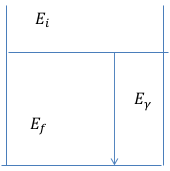
\includegraphics[scale=0.4]{ch7/image1}
	\captionof{figure}{ }
	\end{wrapfigure}
La \textbf{radioactivité $\gamma$} résulte de la transition d'un état d'énergie initial $E_i$ vers un état final
d'énergie $E_f$ avec émission d'un photon. Souvent, l'état final est le fondamental mais ce n'est pas toujours
le cas. Comme les $\gamma$ sont produit par transition électromagnétique, la théorie de \textsc{Fermi} sera 
d'application.\\
 
 
Une fois n'est pas coutume, partons de la conservation de l'énergie et de l'impulsion. Initialement, 
nous avons un noyau d'énergie $E_i$ au repos ($\vec{p_i}=\vec 0$). Finalement nous avons un noyau 
d'énergie $E_f$, d'impulsion $\vec p_r$ (impulsion de recul) et un photon d'énergie $E_\gamma$ 
d'impulsion $\vec p_\gamma$. Par conservation de l'énergie
\begin{equation}
E_i = E_f+E_r+E_\gamma
\end{equation}
où $E_r$ est l'énergie de recul. Par conservation de l'impulsion
\begin{equation}
\vec p_r = -\vec{p_\gamma}
\end{equation}
En en déduit l'énergie de recul
\begin{equation}
E_r = \dfrac{\vec p_r^2}{2m} = \dfrac{\vec p_\gamma^2}{2m} = \dfrac{E_\gamma^2}{2m}
\end{equation}
où $m$ est la masse du noyau ($\approx Am_N$). On peut factoriser l'énergie de recul
\begin{equation}
E_r =\dfrac{E_\gamma^2}{2m} = E_\gamma\dfrac{E_\gamma}{2m}\ll E_\gamma
\end{equation}
Ceci montre que l'énergie de recul est très petite (car $E_\gamma$ est de maximum 20 MeV ce qui
est fort petit par rapport à $mc^2$). En pratique, on la négligera : $E_i = E_f+E_\gamma$.
 
\begin{center}
	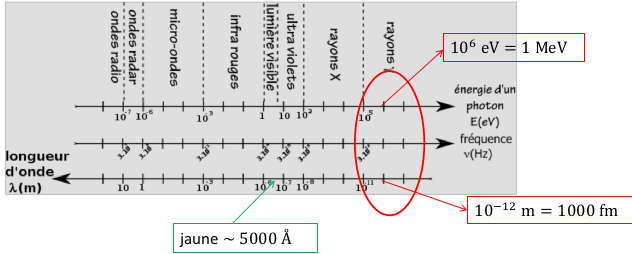
\includegraphics[scale=0.4]{ch7/image2}
	\captionof{figure}{ }
\end{center}
L'ordre de grandeur en physique nucléaire pour l'énergie d'un photon est de l'ordre du MeV, ce qui 
correspond aux rayons $\gamma$.  La longueur d'onde pour $E_\gamma$ = 1 MeV est de
\begin{equation}
\lambda_\gamma = \frac{2\pi}{k_\gamma} = \frac{2\pi \hbar c}{E_\gamma} \approx 1200\ \text{fm}
\end{equation}


\section{Hamiltonien d'interaction nucléons-photon}
L'hamiltonien d'interaction photon-noyau s'écrit 
\begin{equation}
H_{int} \propto H_e a^\dagger
\end{equation}
où $a^\dagger$ est l'opérateur de création d'un photon et $H_e$, l'hamiltonien d'émission d'un photon.
Celui-ci s'écrit (on espère que le développement ci-dessous ne comportera qu'un nombre limité de termes)
\begin{equation}
H_e(\vec{k}_\gamma) = -\sum_{\lambda\mu\sigma} q^\sigma \alpha_\lambda^\sigma \mathcal{M}_\mu^{\sigma\lambda}
(\vec{r}_i)D^\lambda_{\mu q}(\Omega_\gamma)
\end{equation}
Il s'agit d'une factorisation photon-nucléons. On retrouve les termes suivants
\begin{itemize}
\item[$\bullet$] Indice $\sigma$. Soit électrique, soit magnétique. On parle d'équations de \textsc{Maxwell}, les
calculs font apparaître ces deux termes.
\item[$\bullet$] La polarisation du photon. Le photon est de spin entier et possède trois projection, 
$0, \pm1$ mais la projection 0 est interdite. La projection est la polarisation $q$. 
\item[$\bullet$] L'ordre du multipole $\lambda$ (varie de 1 à l'infini, mais en pratique $\lambda=1,2$)
\item[$\bullet$] L'indice $\mu$ est compris entre $-\lambda$ et $+\lambda$
\item[$\bullet$] La fonction de \textsc{Wigner} $D_{\mu q}^\lambda(\Omega_\gamma)$ où $\Omega_\gamma$ est 
l'angle d'émission du photon. 
\item[$\bullet$] Les opérateurs multipolaires $\mathcal{M}_\mu^{\sigma\lambda}(\vec{r}_i)$ qui dépendent des
coordonnées $\vec{r_i}$ est nucléons.
\item[$\bullet$]\begin{equation}
\alpha_\lambda^E = \frac{(ik_\lambda)^\lambda}{(2\lambda-1)!!}\sqrt{\dfrac{4\pi(\lambda+1)}{2\lambda(2\lambda+1)}}
\end{equation}
avec $\alpha_\lambda^M = -i\alpha^E_\lambda$.
\end{itemize}


Intéressons-nous aux \textbf{opérateurs multipolaires} $\mathcal{M}_\mu^{\sigma\lambda}$ dans l'approximation
des grandes longueurs d'ondes ($kr \ll 1$). Il en existe deux types : électrique et magnétique.\\

\retenir{\textbf{opérateur multipolaire électrique}\begin{equation}
\mathcal{M}_\mu^{E\lambda}e\sum_i\left(\frac{1}{2}-t_{iz}\right)r_i^\lambda Y_\lambda^\mu (\Omega_{ri})
\end{equation}}\ \\

C'est le plus important, on somme sur tous les nucléons et on voit apparaître un facteur d'isospin car 
seulement les protons interagissent avec l'interaction électromagnétique (la contribution des neutrons dans
cette somme doit être nulle. Le facteur d'isospin vaut +1 pour les protons et zéro pour les neutrons).\ \\

Il y a aussi l'opérateur multipolaire magnétique
\begin{equation}
\mathcal{M}_\mu^{M\lambda} = \mu_N\sum_i[\vec\nabla(r^\lambda Y_\lambda^\mu(\Omega_r)]_{r=r_i}.\left(
\frac{2g_{li}}{\lambda+1}\vec{L}_i+g_{si}\vec{S}_i\right)
\end{equation}
où $\mu_N = (e\hbar)/(m_Nc)$ est le magnéton de \textsc{Bohr}. Un peu plus compliqué. Celui-ci contient des termes
venant du champ magnétiques qui sont moins habituels. On somme toujours sur les nucléons mais on voit apparaître le
gradient. C'est un vecteur qu'on prend en produit scolaire avec un autre vecteur qui contient le moment cinétique
orbital et le spin intrinsèque pour chaque nucléon. Le terme en $\vec L_i$ n'interagit que sur les protons. 
\begin{equation}
g_{li} = \frac{1}{2}-t_{iz}
\end{equation}
Pour le spin, c'est plus compliqué : $g_{si}$ contient un terme associé au proton et un au neutron
\begin{equation}
g_{si} = g_p\left(\frac{1}{2}-t_{iz}\right)+g_n\left(\frac{1}{2}+t_{iz}\right)
\end{equation}
où $g_p=5.586$ et $g_n=-3.826$ sont des facteur gyromagnétiques déterminés expérimentalement\footnote{Pour une
particule élémentaire, ce facteur vaut exactement 2.}. Notons que pour $\lambda = 0$, il n'y a pas de transition monopolaire.Une étude de la \textbf{parité} est donnée au \textit{slide 106} (je n'ai pas de notes\dots Si 
quelqu'un pouvait compléter).


\section{Probabilité de transition}
\subsection{A. Distributions angulaires}
Considérons comme état initial la fonction d'onde du noyau $\Psi^{J_iM_i\pi_i}$ et 0 photon et comme état final
la fonction d'onde du noyau $\Psi^{J_fM_f\pi_f}$ et 1 photon.La probabilité de transition est donnée par la
règle d'or de \textsc{Fermi}
\begin{equation}
dw_{if} = \frac{2\pi}{\hbar}\left|\bra{1,\Psi^{J_fM_f\pi_f}}H_{int}\ket{0,\Psi^{J_iM_i\pi_i}}\right|^2d\rho(E_i)
\end{equation}
où $d\rho(E_i)=\frac{d\vec k_\gamma}{dE}=\frac{k_\gamma^2}{\hbar c}d\Omega_\gamma$ est la densité d'état avec
$\Omega_\gamma$ l'angle d'émission du photon. \\

Considérons l'Hamiltonien d'interaction écrit à l'aide de l'opérateur élévateur
\begin{equation}
H_{int} = H_ea_{kq}^\dagger
\end{equation}
où $H_e(k,\epsilon_{kq}) = -\sum_{\lambda\mu\sigma}(-1)^\lambda q^\sigma a_\lambda^\sigma \mathcal{M}_\mu^{
\sigma\lambda}D_{\mu-q}^\lambda(\Omega_\gamma)$.\\

Pour l'émission d'un photon de nombre d'onde $k_y$ nous avons
\begin{equation}
\bra{1}a_{kq}^\dagger\ket{0} = \delta(k-k_\gamma)
\end{equation}
En intégrant sur $dk$ ce résultat
\begin{equation}
\int dk\ \bra{1}a_{kq}^\dagger\ket{H_e(k\epsilon_{kq})} = H_e(k_\gamma,\epsilon_{kq})
\end{equation}
Il est possible de réécrire la distribution angulaire $w_{if}$
\begin{equation}
\frac{dw_{if}}{d\Omega_\gamma} = \sum_q\left|\sum_{\lambda\mu\lambda}(-1)^\lambda q^\sigma\alpha_\lambda^\sigma
\underbrace{\bra{\Psi^{J_fM_f\pi_f}}\mathcal{M}_\mu^{\sigma\lambda}\ket{\Psi^{J_iM_i\pi_i}}}_{\text{nucléons}}
\underbrace{D_{\mu-q}^\lambda(\Omega_\gamma)}_{\text{photon}}\right|^2
\end{equation}
Après intégration sur $\Omega_\gamma$, on trouve
\begin{equation}
w_{J_iM_i\pi_i\to J_fM_f\pi_f} \approx \sum_{\lambda\mu\sigma} |\alpha_\lambda^\sigma|^|\left|
\bra{\Psi^{J_fM_f\pi_f}}\mathcal{M}_\mu^{\sigma\lambda}\ket{\Psi^{J_iM_i\pi_i}}\right|^2
\end{equation}
Cette somme porte sur les trois multipôles :
\begin{itemize}
\item[$\bullet$] $\sigma = E$ (électrique) ou $M$ (magnétique)
\item[$\bullet$] $\lambda=$ ordre du multipôle (de 0 à $\infty$)
\item[$\bullet$] $\mu =$ projection $-\lambda\leq \mu\leq\lambda$
\end{itemize}\ 

Heureusement en pratique, seul un petit nombre de terme de cette somme contribue grâces notamment aux 
règles de sélections mais aussi via le développement en puissance de $k_\gamma R$ ($\ll 1$).

\subsection{B. Règles de sélection}
Pas de notes (tout fait au tableau\dots) pour cette section et les trois suivantes. En demander!
\subsection{C. Probabilité de transition totale}
\subsection{D. Largeur gamma}
\subsection{F. Cas particuliers : transition $E_1$ dans les noyaux $N=Z$}
Considérons l'opérateur $E1$
\begin{equation}
\mathcal{M}_\mu^{E1} = e\sum_i\left(\frac{1}{2}-t_{iz}\right)r_iY_1^\mu(\Omega_{ri})\propto \sum_i
\left(\frac{1}{2}-t_{iz}\right)\vec{r}_{i\mu}
\end{equation}

Dans la coordonnée $\vec{R}$, on doit supprimer le centre de masse. En effet, si on prend le premier
facteur $1/2$, le centre de masse est défini de sorte à ce que cette somme soit nulle. Il ne reste donc
que la contribution du terme en isospin
\begin{equation}
\mathcal{M}_\mu^{E1} \propto sum_i\left(\frac{1}{2}-t_{iz}\right)(\vec{r}_{i\mu}-\vec{R}_{c.m.,\mu})
\propto -sum_i-t_{iz}(\vec{r}_{i\mu}-\vec{R}_{c.m.,\mu})
\end{equation}
Il s'agit d'un OTI de rang 1 dans l'espace des isospin. Pour un noyau où $N=Z$, $T_Z=0, T\approx0$. Le 
coefficient de CG peut se calculer via le théorème de \textsc{Wigner-Eckart}
\begin{equation}
\bra{0010}\ket{00} = 0
\end{equation}
Les transitions $E1$, qui sont en principe dominantes, sont ici interdites. Cependant, comme $T$ n'est 
pas un bon nombre quantique exact, les largeurs $E_1$ sont en générales non-nulles.





\subsection{G. Unités Weisskopf}
Il s'agit d'unités souvent utilisées. L'idée n'est pas de faire un calcul savant de la probabilité de transition
mais un certain \textit{feeling} pour avoir un ordre de grandeur. En supposant qu'un seul nucléons participe à
la transition, elles permettent donc d'estimer très simplement les probabilités de transitions réduites. Les
définitions de cette unité sont données \textit{slide 114}.

\subsection{F. Exemples}
Serait fait lorsque les sections \textsc{B,C,D,F} seront faites, pas de sens avant.





\subsection{I. États isométriques}
Les états isométriques sont des états de longue durée de vie. Comme $\tau\propto 1/W$, il faut que
$W$ soit petit. Rappelons l'expression de $W$
\begin{equation}
W(\sigma,\lambda) \propto E_\gamma^{2\lambda+1}\left|\bra{\Psi^{J_f\pi_f}}\mathcal{M}^{\sigma\lambda}\ket{
\Psi^{J_i\pi_i}}\right|^2
\end{equation}
Pour avoir une longue durée de vie, il faut donc que $E_\gamma$ soit petit et donc $\lambda$ grand, impliquant
que $J_f-J_i$ soit être important. De façon assez surprenante, il existe parfois des durées de vies plus 
longue que le fondamental.

